\chapter{Examples}
\label{app:examples}
We select five different mammograms and show the predictions made by our different models (next page).
% Examples: img_5_9_1_LO, img_3_4_1_LCC, img_186_251_1_RCC, img_251_334_1_LO, img_377_522_1_LCC

\newpage
\section{Example 1}
\begin{figure}[h]
	\centering
	\begin{subfigure}{0.2\textwidth}
		\centering
			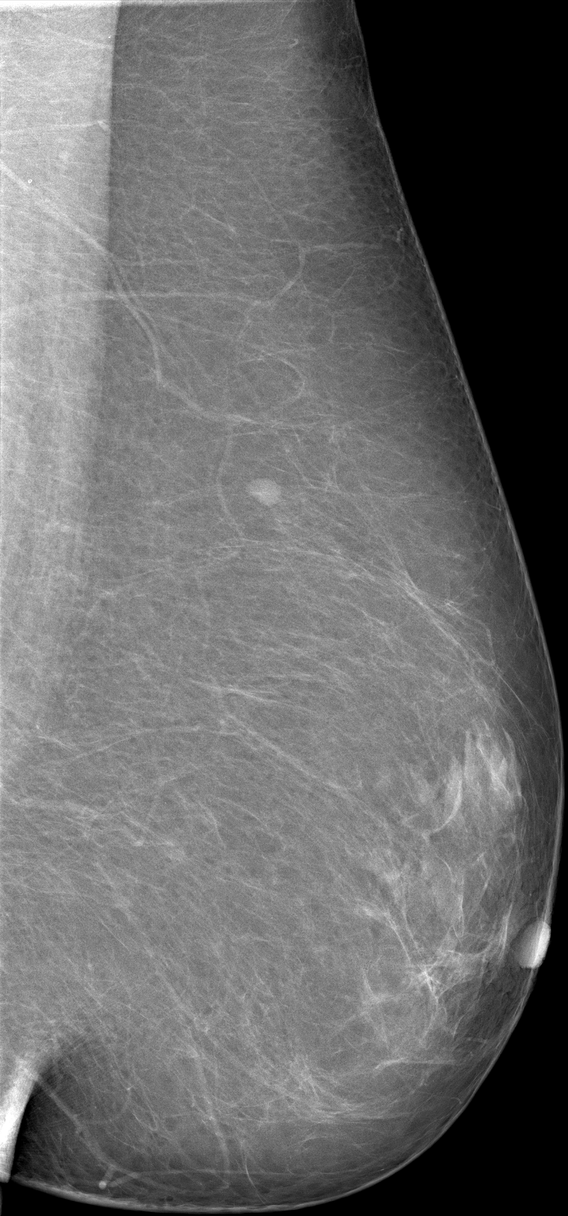
\includegraphics[width=\textwidth]{plots/examples/mammogram_1.png}
         \caption{Mammogram}
	\end{subfigure}
	\quad
	\begin{subfigure}{0.2\textwidth}
		\centering
			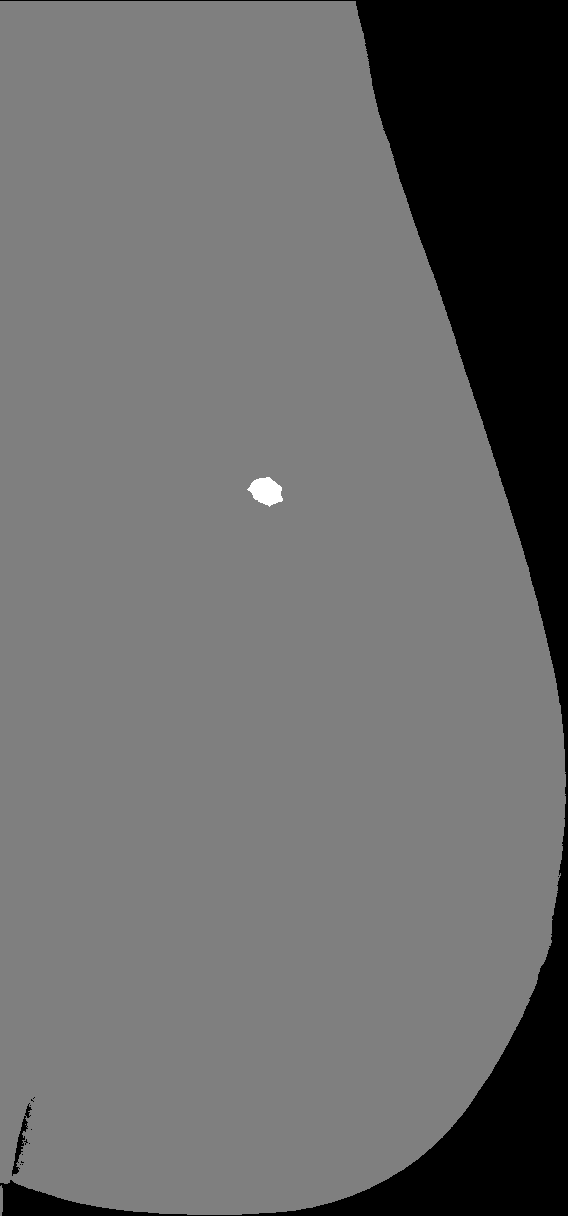
\includegraphics[width=\textwidth]{plots/examples/label_1.png}
         \caption{Ground truth}
	\end{subfigure}
	\caption[Example 1]{Example 1}
\end{figure}

\begin{figure}[h!]
	\centering
	\begin{subfigure}{0.195\textwidth}
		\centering
			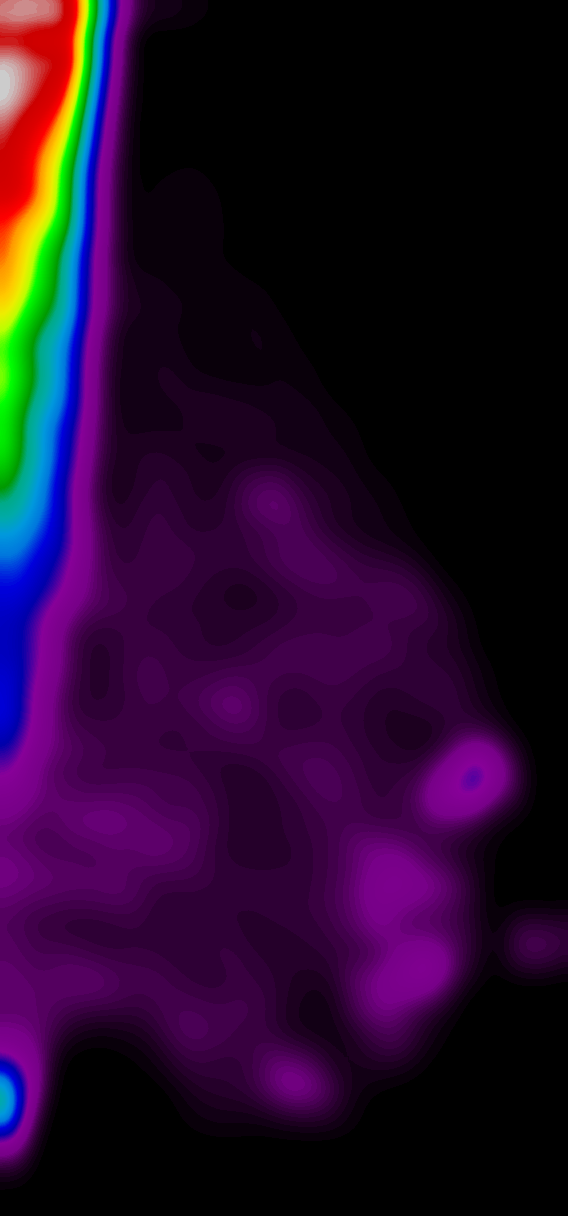
\includegraphics[width=\textwidth]{plots/examples/example1_probs_1_1.png}
		\caption{Experiment 1.1}
    \end{subfigure}
	\begin{subfigure}{0.195\textwidth}
		\centering
			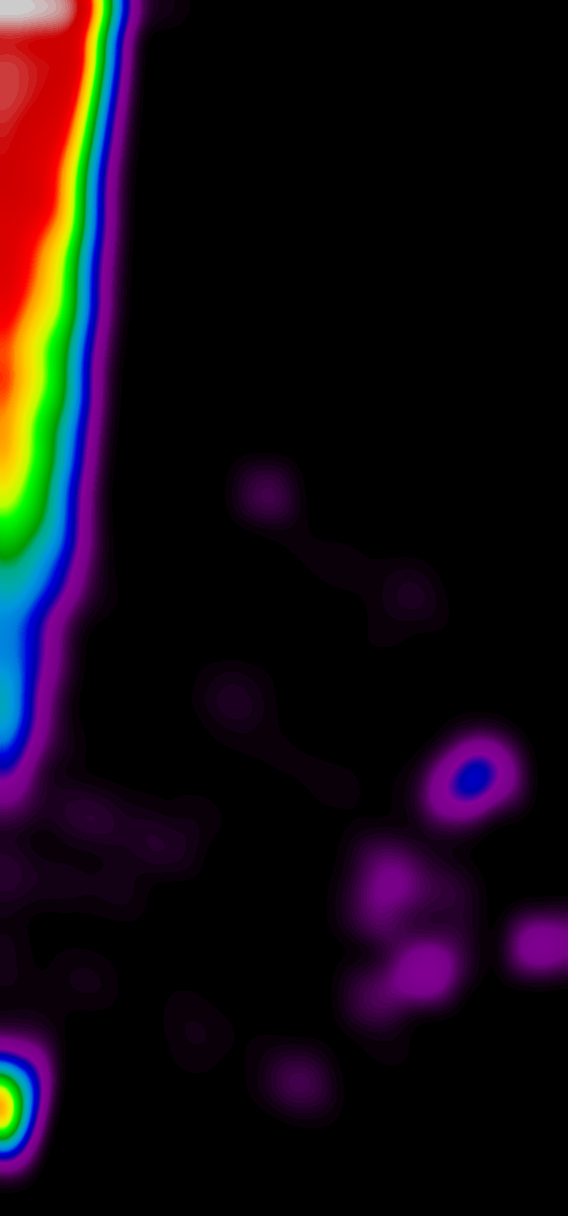
\includegraphics[width=\textwidth]{plots/examples/example1_probs_1_2.png}
		\caption{Experiment 1.2}
    \end{subfigure}
	\begin{subfigure}{0.195\textwidth}
		\centering
			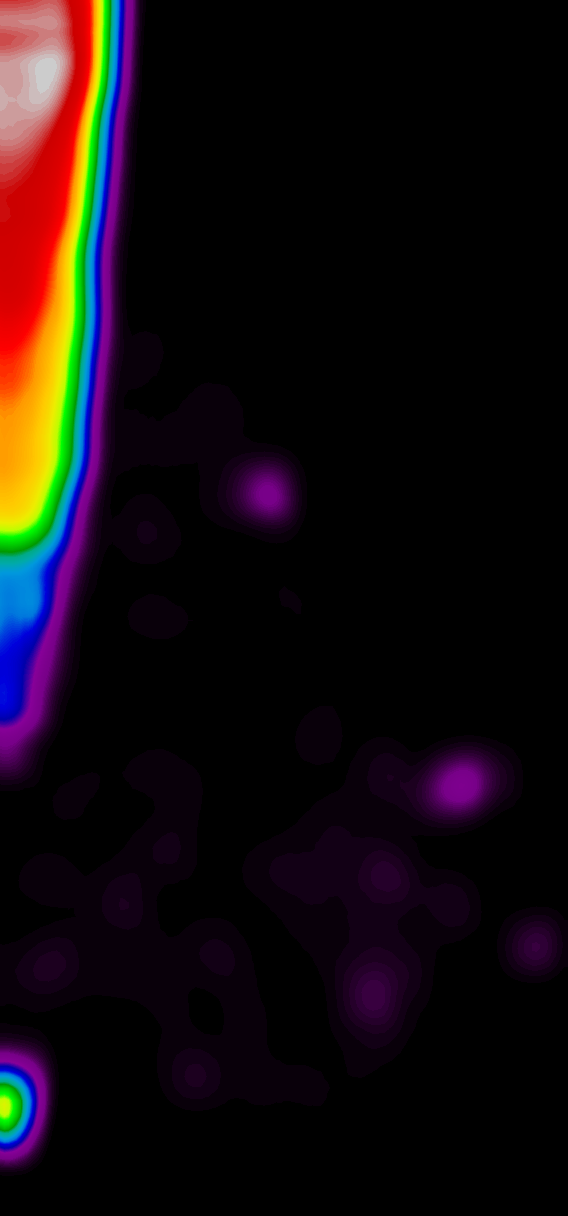
\includegraphics[width=\textwidth]{plots/examples/example1_probs_1_3.png}
		\caption{Experiment 1.3}
    \end{subfigure}
	\begin{subfigure}{0.195\textwidth}
		\centering
			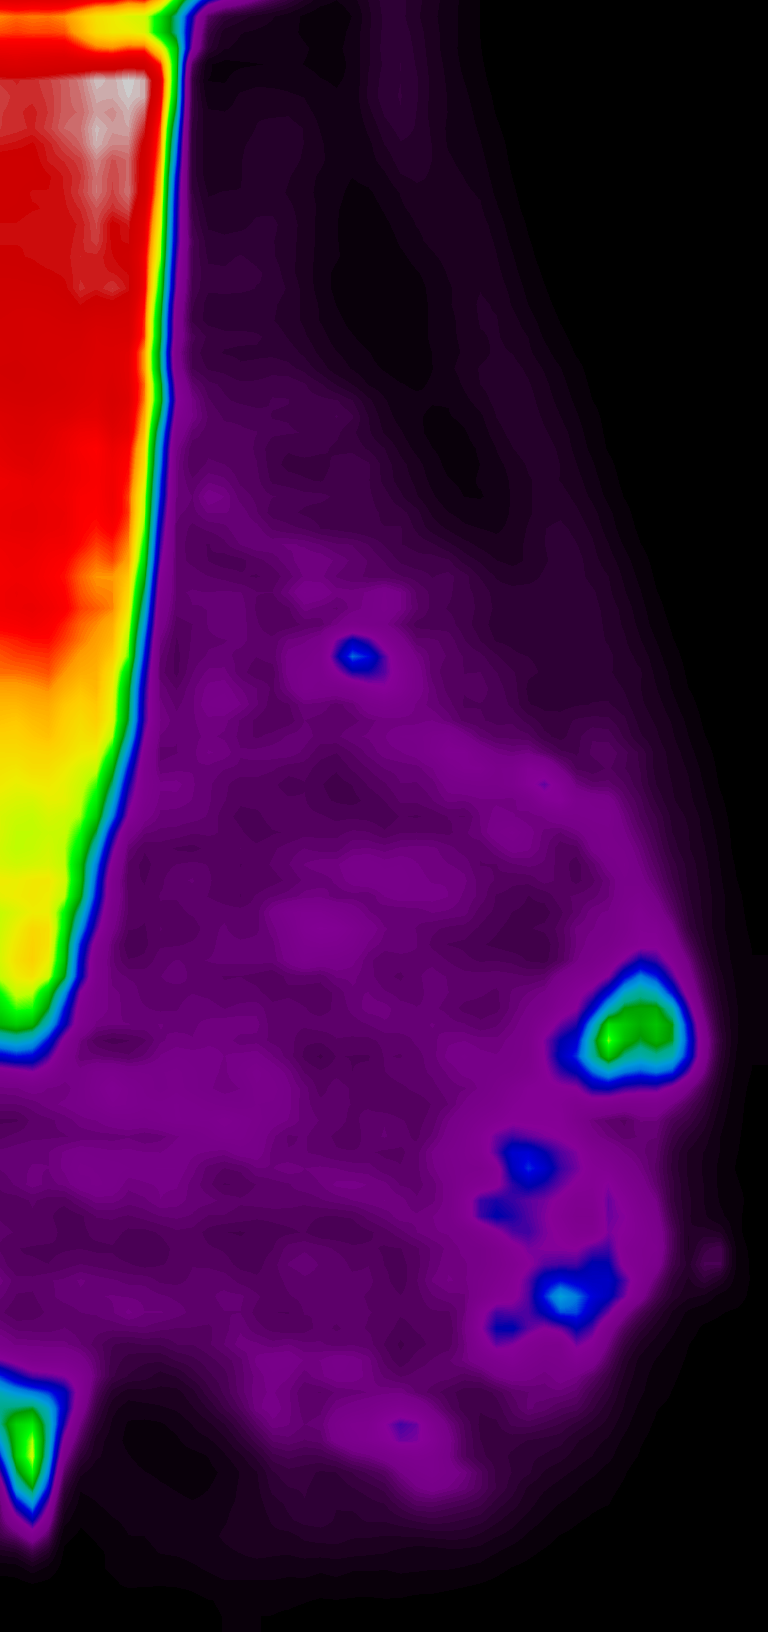
\includegraphics[width=\textwidth]{plots/examples/example1_probs_2.png}
		\caption{Experiment 2}
    \end{subfigure}
    \begin{subfigure}{0.195\textwidth}
		\centering
			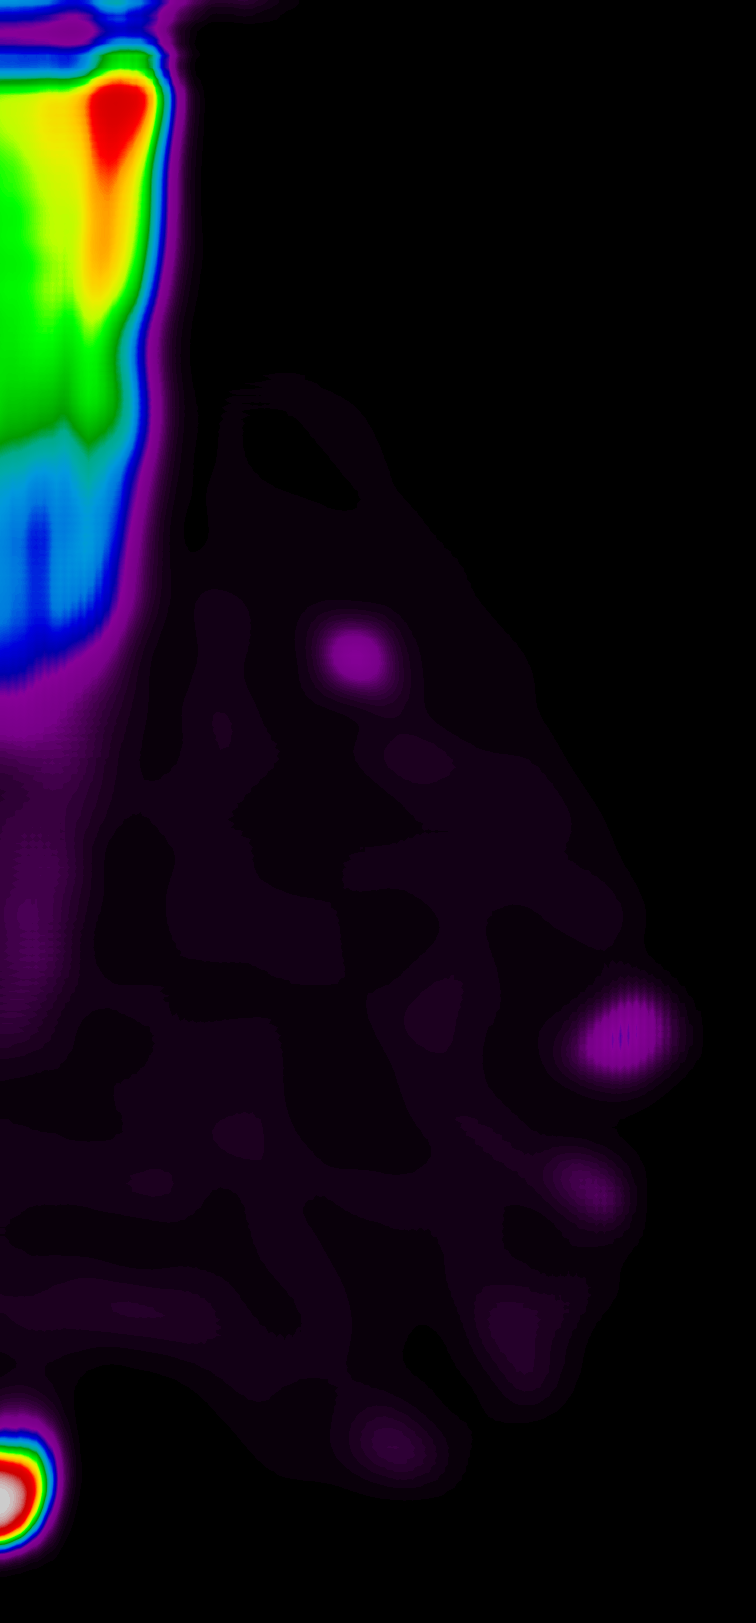
\includegraphics[width=\textwidth]{plots/examples/example1_probs_3.png}
		\caption{Experiment 3}
    \end{subfigure}
	\caption[Predictions for example 1]{Predicted probabilitites for example 1.}
\end{figure}

\newpage
\section{Example 2}
\begin{figure}[h]
	\centering
	\begin{subfigure}{0.2\textwidth}
		\centering
			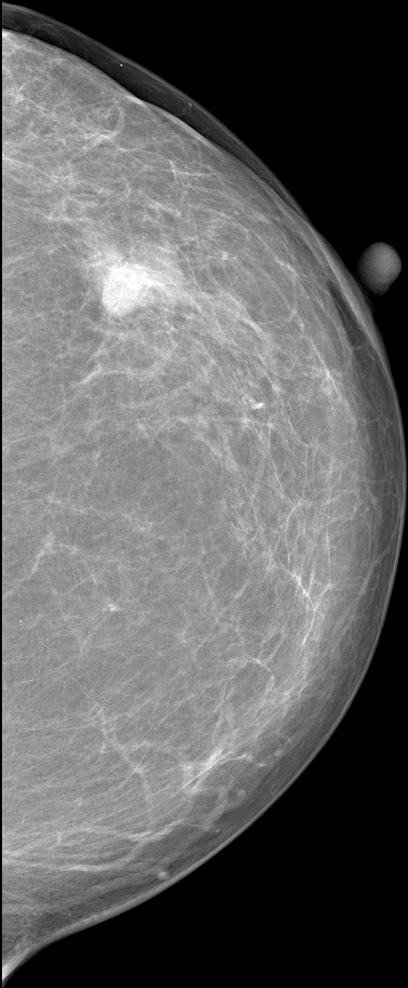
\includegraphics[width=\textwidth]{plots/examples/mammogram_2.png}
		\caption{Mammogram}
	\end{subfigure}
	\quad
	\begin{subfigure}{0.2\textwidth}
		\centering
			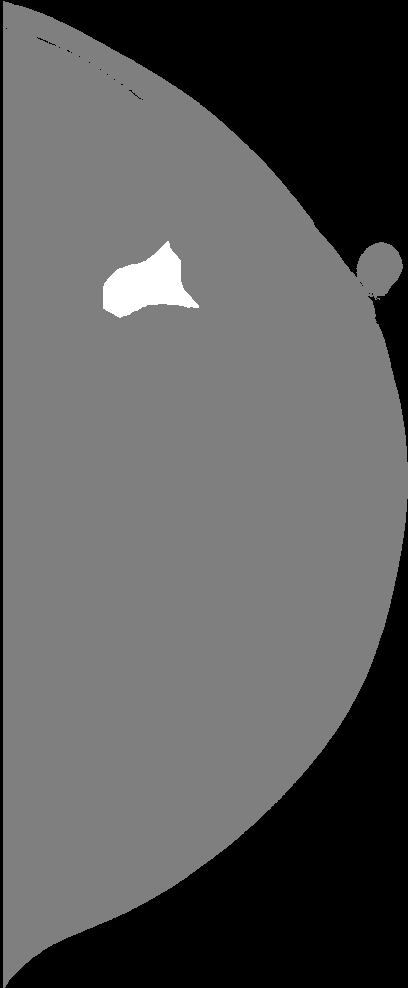
\includegraphics[width=\textwidth]{plots/examples/label_2.png}
         \caption{Ground truth}
	\end{subfigure}
	\caption[Example 2]{Example 2}
\end{figure}

\begin{figure}[h!]
	\centering
	\begin{subfigure}{0.195\textwidth}
		\centering
			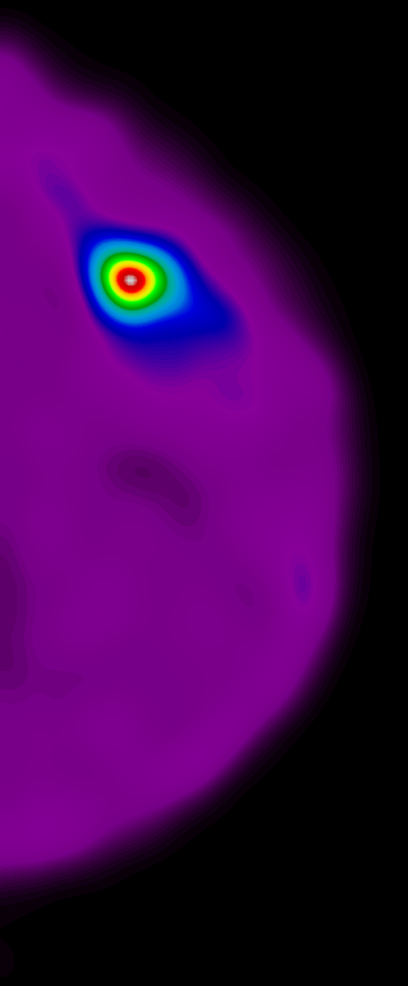
\includegraphics[width=\textwidth]{plots/examples/example2_probs_1_1.png}
		\caption{Experiment 1.1}
    \end{subfigure}
	\begin{subfigure}{0.195\textwidth}
		\centering
			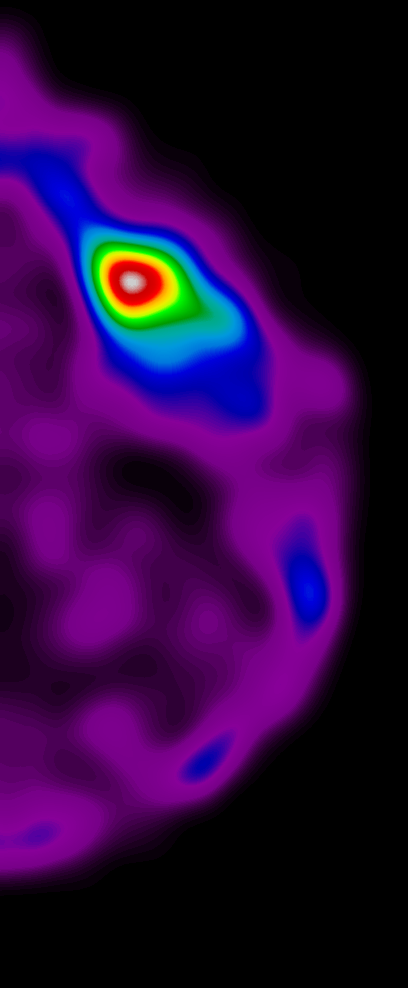
\includegraphics[width=\textwidth]{plots/examples/example2_probs_1_2.png}
		\caption{Experiment 1.2}
    \end{subfigure}
	\begin{subfigure}{0.195\textwidth}
		\centering
			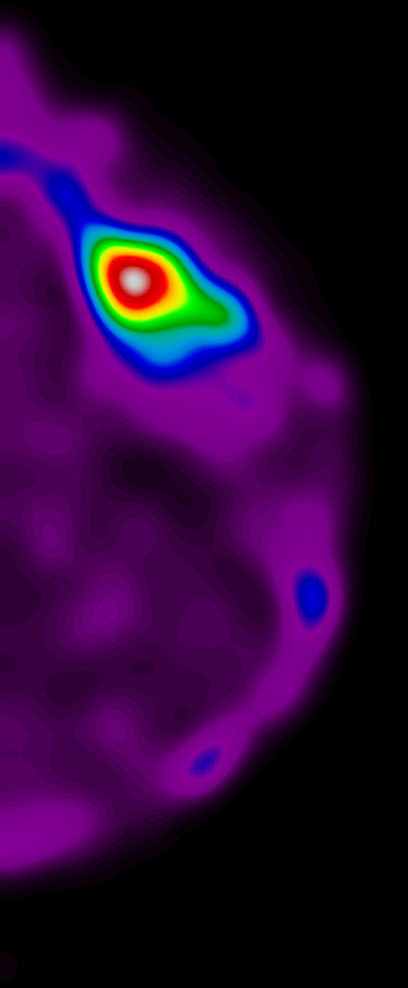
\includegraphics[width=\textwidth]{plots/examples/example2_probs_1_3.png}
		\caption{Experiment 1.3}
    \end{subfigure}
	\begin{subfigure}{0.195\textwidth}
		\centering
			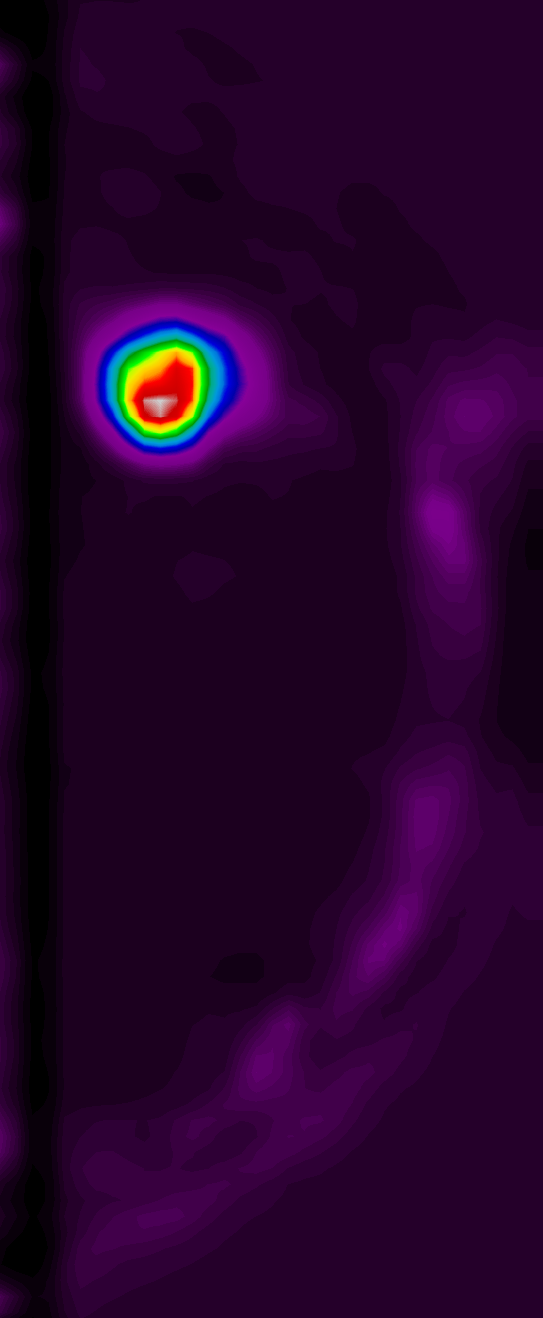
\includegraphics[width=\textwidth]{plots/examples/example2_probs_2.png}
		\caption{Experiment 2}
    \end{subfigure}
    \begin{subfigure}{0.195\textwidth}
		\centering
			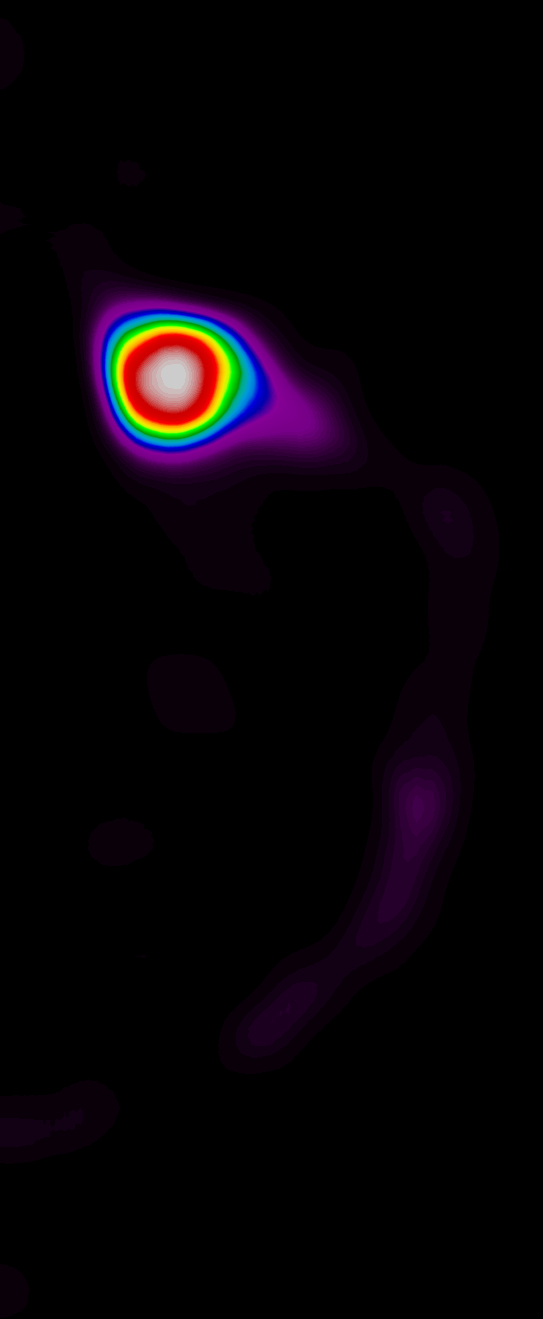
\includegraphics[width=\textwidth]{plots/examples/example2_probs_3.png}
		\caption{Experiment 3}
    \end{subfigure}
	\caption[Predictions for example 2]{Predicted probabilitites for example 2.}
\end{figure}

\newpage
\section{Example 3}
\begin{figure}[h]
	\centering
	\begin{subfigure}{0.2\textwidth}
		\centering
			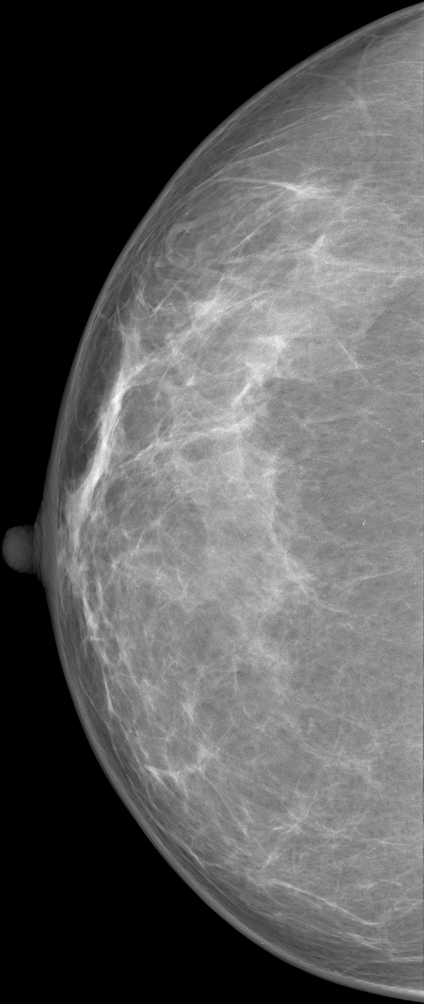
\includegraphics[width=\textwidth]{plots/examples/mammogram_3.png}
         \caption{Mammogram}
	\end{subfigure}
	\quad
	\begin{subfigure}{0.2\textwidth}
		\centering
			
\includegraphics[width=\textwidth]{plots/examples/label_3.png}
         \caption{Ground truth}
	\end{subfigure}
	\caption[Example 3]{Example 3}
\end{figure}

\begin{figure}[h!]
	\centering
	\begin{subfigure}{0.195\textwidth}
		\centering
			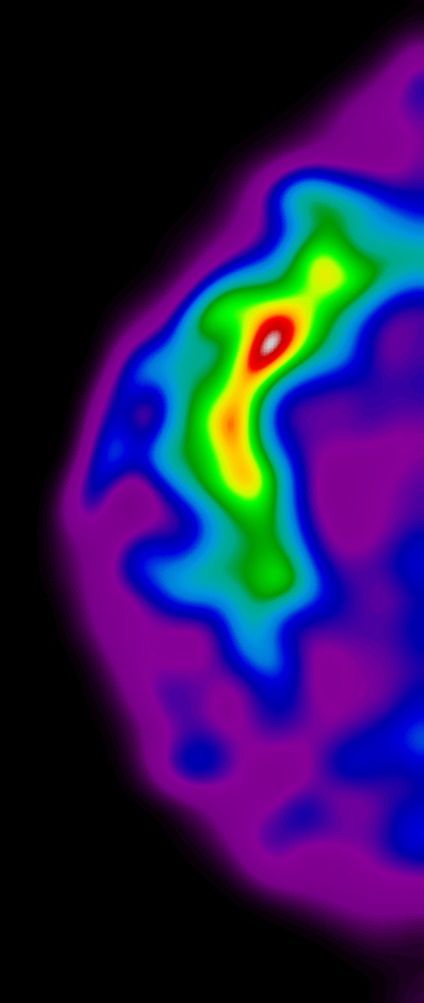
\includegraphics[width=\textwidth]{plots/examples/example3_probs_1_1.png}
		\caption{Experiment 1.1}
    \end{subfigure}
	\begin{subfigure}{0.195\textwidth}
		\centering
			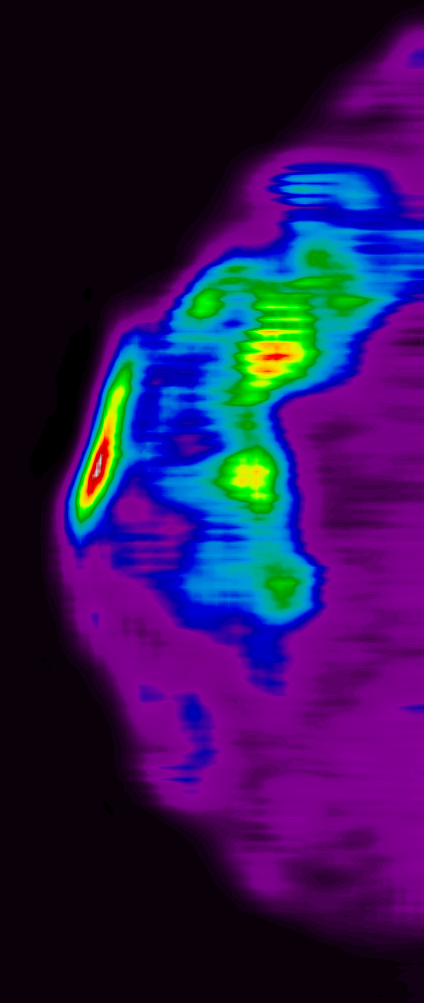
\includegraphics[width=\textwidth]{plots/examples/example3_probs_1_2.png}
		\caption{Experiment 1.2}
    \end{subfigure}
	\begin{subfigure}{0.195\textwidth}
		\centering
			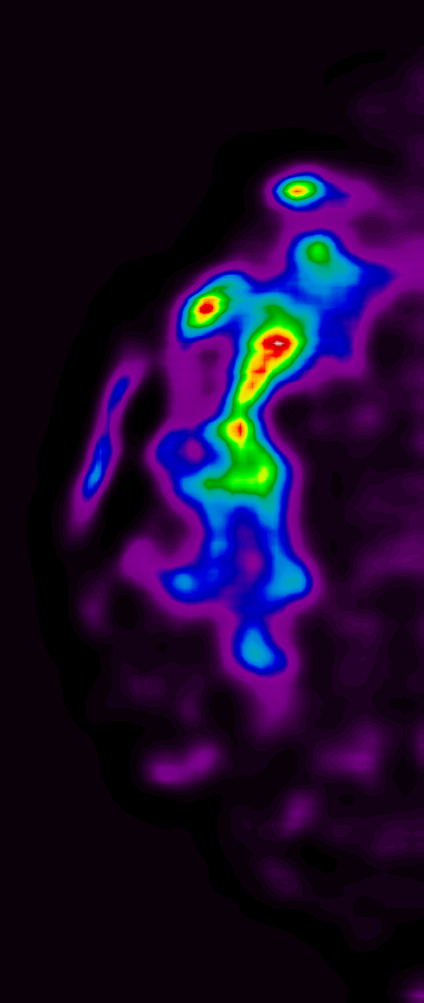
\includegraphics[width=\textwidth]{plots/examples/example3_probs_1_3.png}
		\caption{Experiment 1.3}
    \end{subfigure}
	\begin{subfigure}{0.195\textwidth}
		\centering
			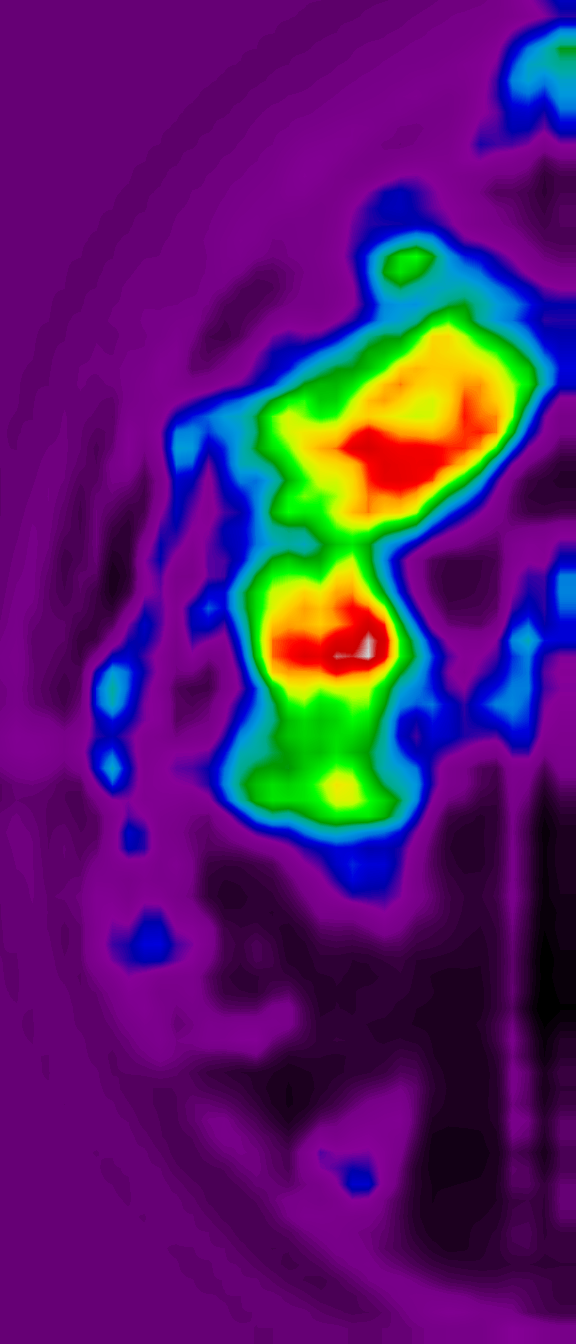
\includegraphics[width=\textwidth]{plots/examples/example3_probs_2.png}
		\caption{Experiment 2}
    \end{subfigure}
    \begin{subfigure}{0.195\textwidth}
		\centering
			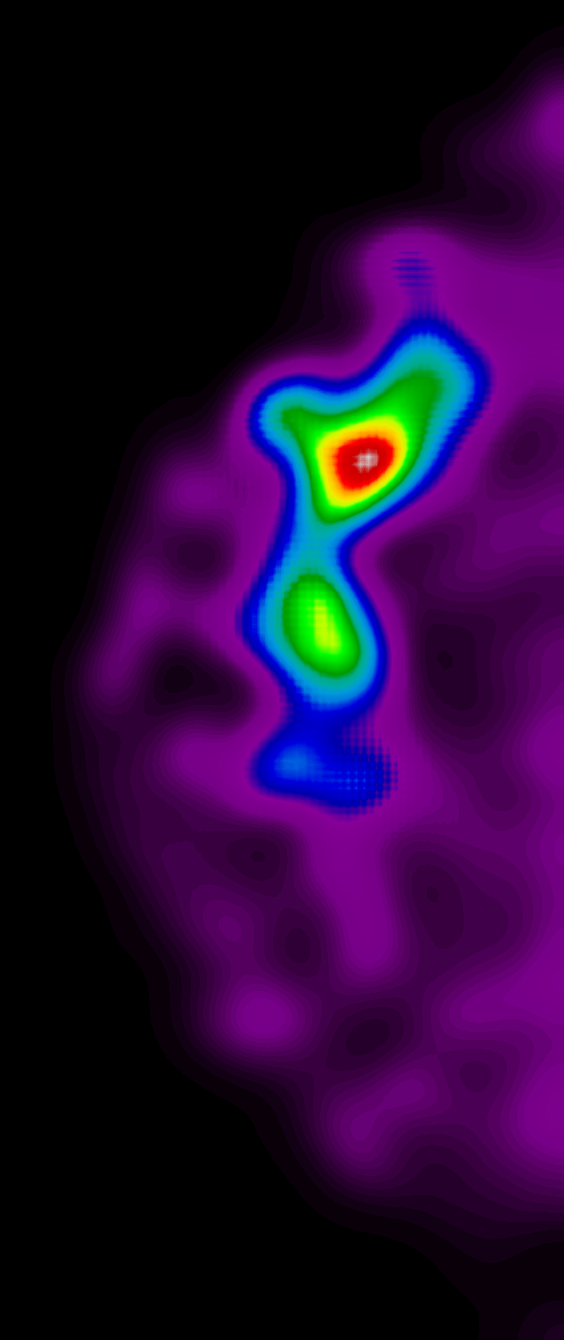
\includegraphics[width=\textwidth]{plots/examples/example3_probs_3.png}
		\caption{Experiment 3}
    \end{subfigure}
	\caption[Predictions for example 3]{Predicted probabilitites for example 3.}
\end{figure}

\newpage
\section{Example 4}
\begin{figure}[h]
	\centering
	\begin{subfigure}{0.2\textwidth}
		\centering
			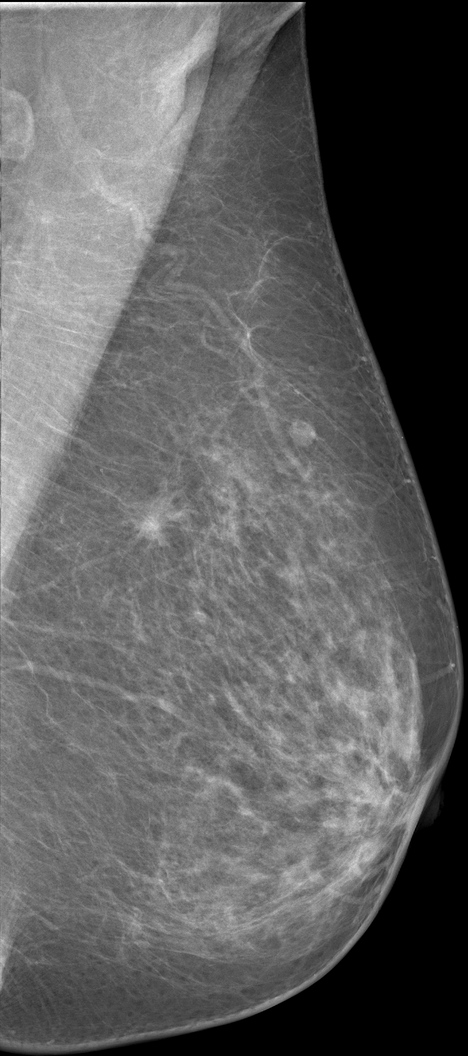
\includegraphics[width=\textwidth]{plots/examples/mammogram_4.png}
         \caption{Mammogram}
	\end{subfigure}
	\quad
	\begin{subfigure}{0.2\textwidth}
		\centering
			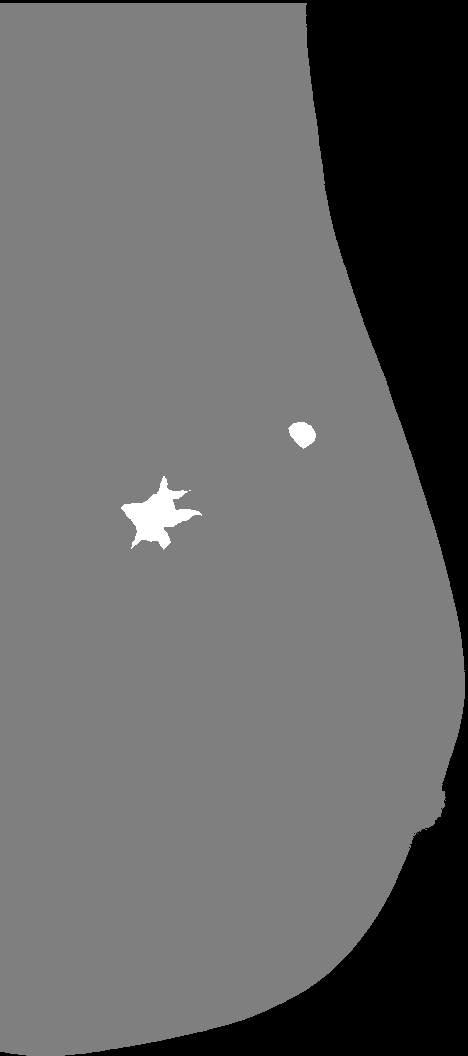
\includegraphics[width=\textwidth]{plots/examples/label_4.png}
         \caption{Ground truth}
	\end{subfigure}
	\caption[Example 4]{Example 4}
\end{figure}

\begin{figure}[h!]
	\centering
	\begin{subfigure}{0.195\textwidth}
		\centering
			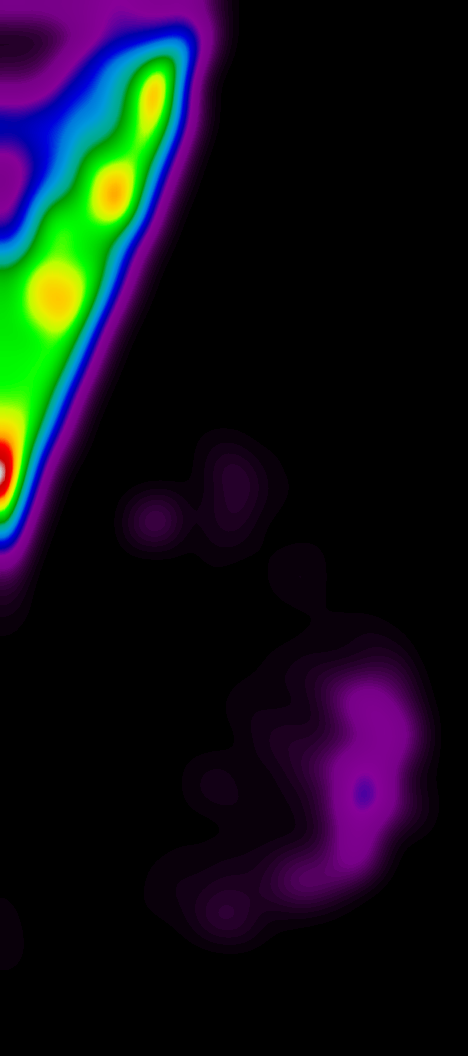
\includegraphics[width=\textwidth]{plots/examples/example4_probs_1_1.png}
		\caption{Experiment 1.1}
    \end{subfigure}
	\begin{subfigure}{0.195\textwidth}
		\centering
			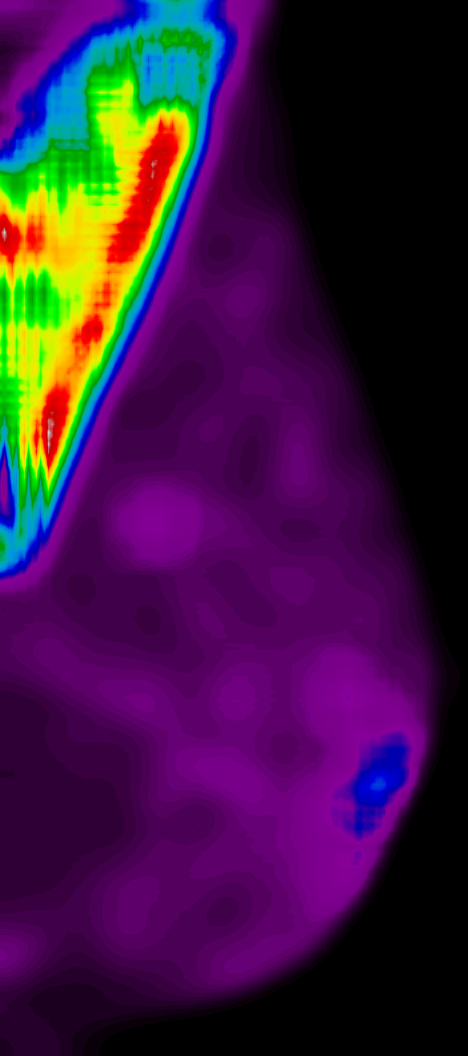
\includegraphics[width=\textwidth]{plots/examples/example4_probs_1_2.png}
		\caption{Experiment 1.2}
    \end{subfigure}
	\begin{subfigure}{0.195\textwidth}
		\centering
			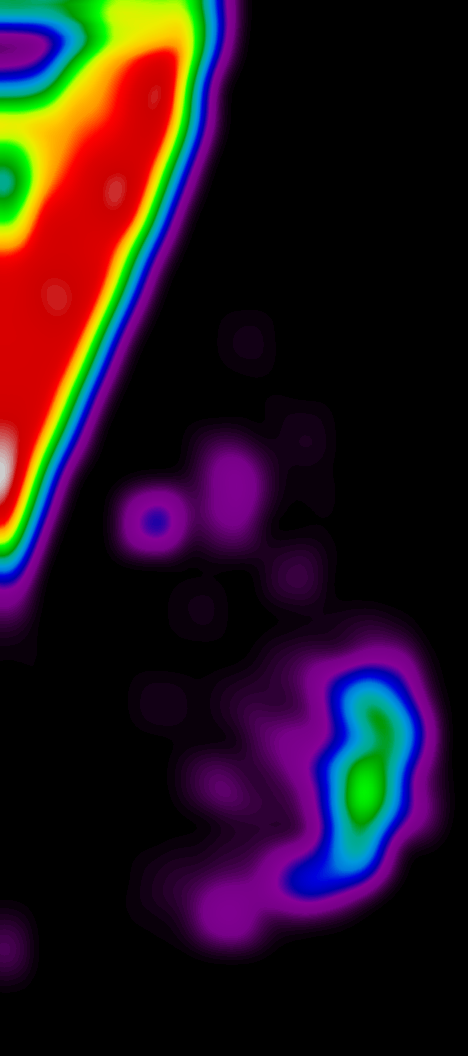
\includegraphics[width=\textwidth]{plots/examples/example4_probs_1_3.png}
		\caption{Experiment 1.3}
    \end{subfigure}
	\begin{subfigure}{0.195\textwidth}
		\centering
			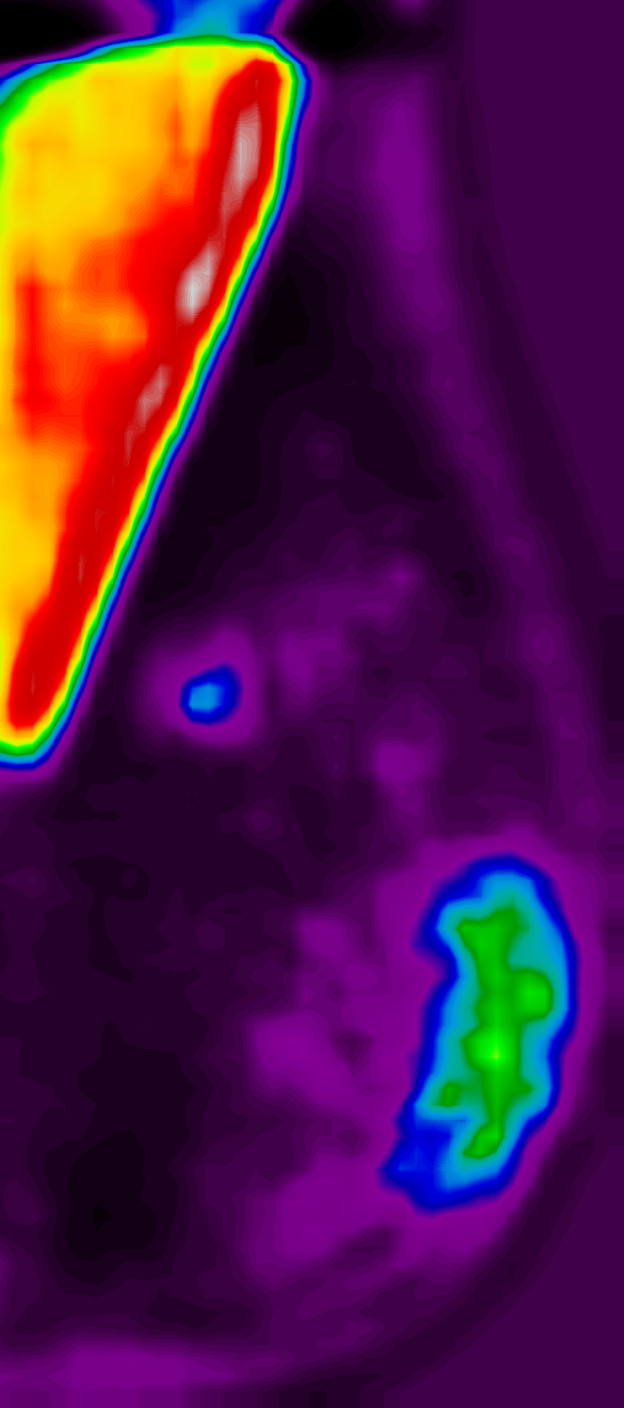
\includegraphics[width=\textwidth]{plots/examples/example4_probs_2.png}
		\caption{Experiment 2}
    \end{subfigure}
    \begin{subfigure}{0.195\textwidth}
		\centering
			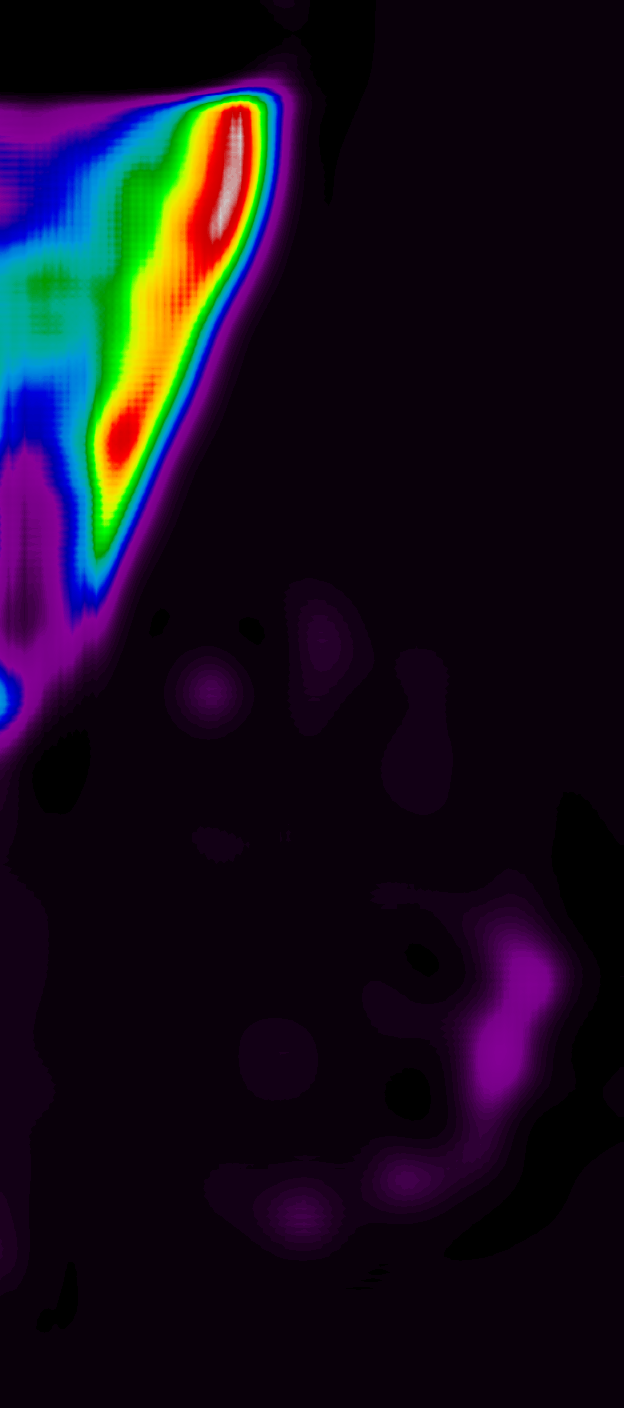
\includegraphics[width=\textwidth]{plots/examples/example4_probs_3.png}
		\caption{Experiment 3}
    \end{subfigure}
	\caption[Predictions for example 4]{Predicted probabilitites for example 4.}
\end{figure}

\newpage
\section{Example 5}
\begin{figure}[h]
	\centering
	\begin{subfigure}{0.2\textwidth}
		\centering
			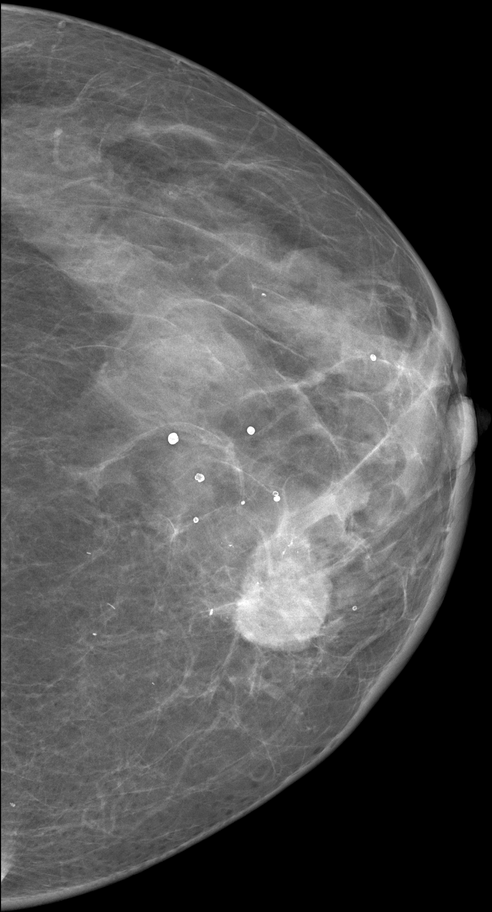
\includegraphics[width=\textwidth]{plots/examples/mammogram_5.png}
         \caption{Mammogram}
	\end{subfigure}
	\quad
	\begin{subfigure}{0.2\textwidth}
		\centering
			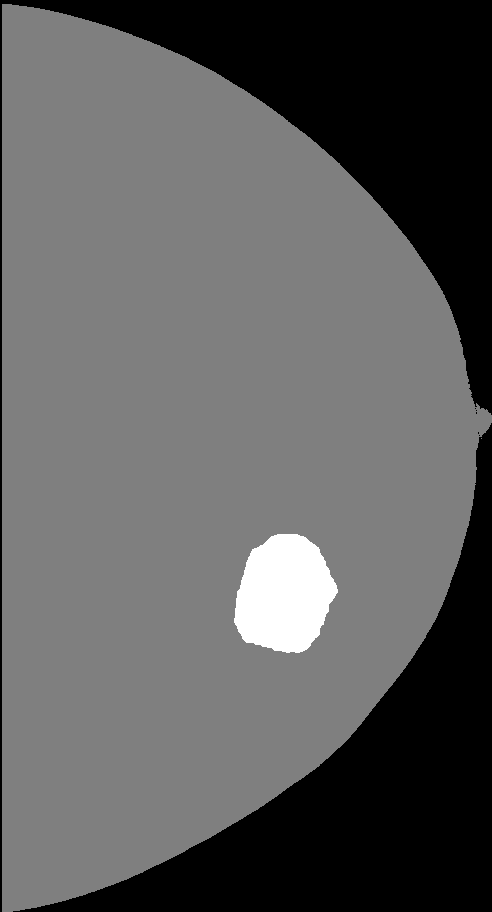
\includegraphics[width=\textwidth]{plots/examples/label_5.png}
         \caption{Ground truth}
	\end{subfigure}
	\caption[Example 5]{Example 5}
\end{figure}

\begin{figure}[h!]
	\centering
	\begin{subfigure}{0.195\textwidth}
		\centering
			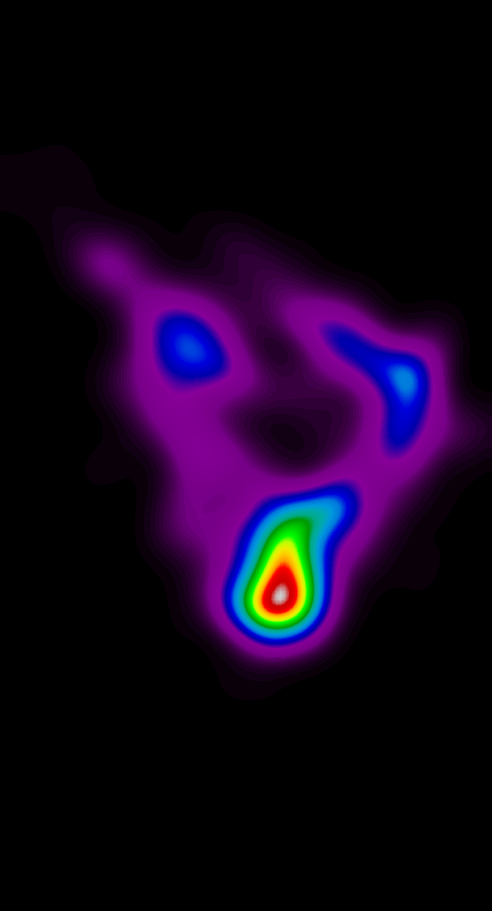
\includegraphics[width=\textwidth]{plots/examples/example5_probs_1_1.png}
		\caption{Experiment 1.1}
    \end{subfigure}
	\begin{subfigure}{0.195\textwidth}
		\centering
			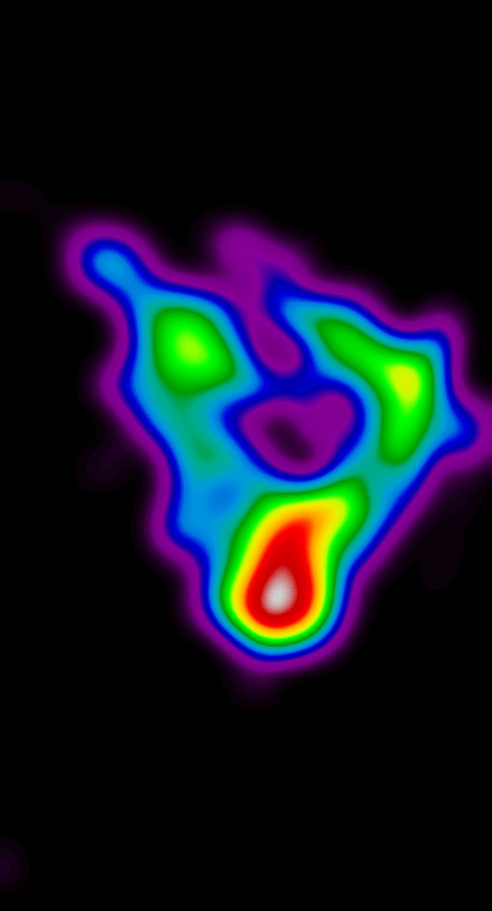
\includegraphics[width=\textwidth]{plots/examples/example5_probs_1_2.png}
		\caption{Experiment 1.2}
    \end{subfigure}
	\begin{subfigure}{0.195\textwidth}
		\centering
        	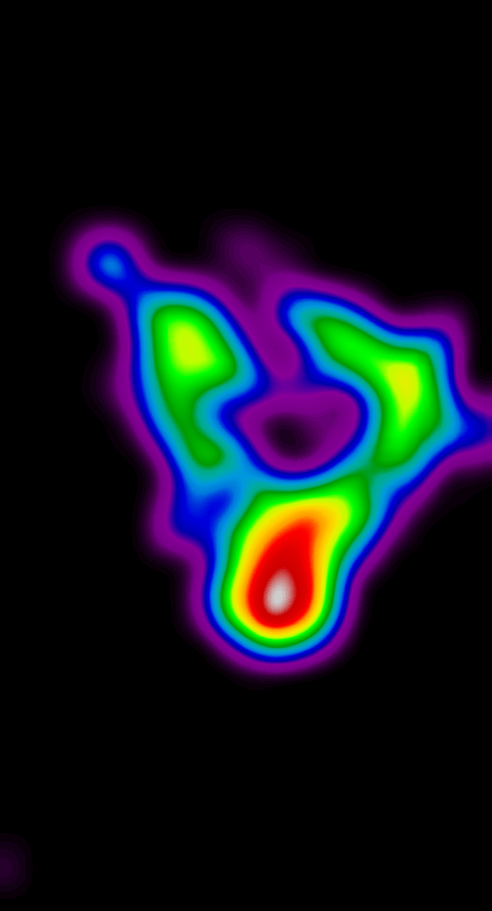
\includegraphics[width=\textwidth]{plots/examples/example5_probs_1_3.png}
		\caption{Experiment 1.3}
    \end{subfigure}
	\begin{subfigure}{0.195\textwidth}
		\centering
			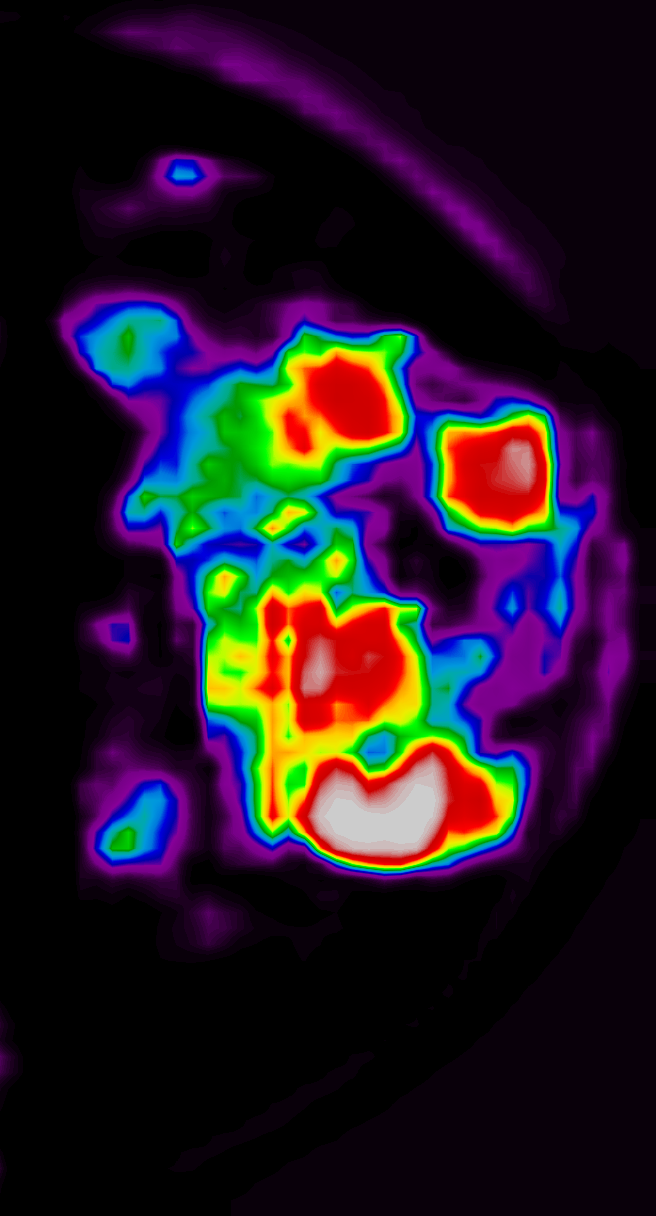
\includegraphics[width=\textwidth]{plots/examples/example5_probs_2.png}
		\caption{Experiment 2}
    \end{subfigure}
    \begin{subfigure}{0.195\textwidth}
		\centering
			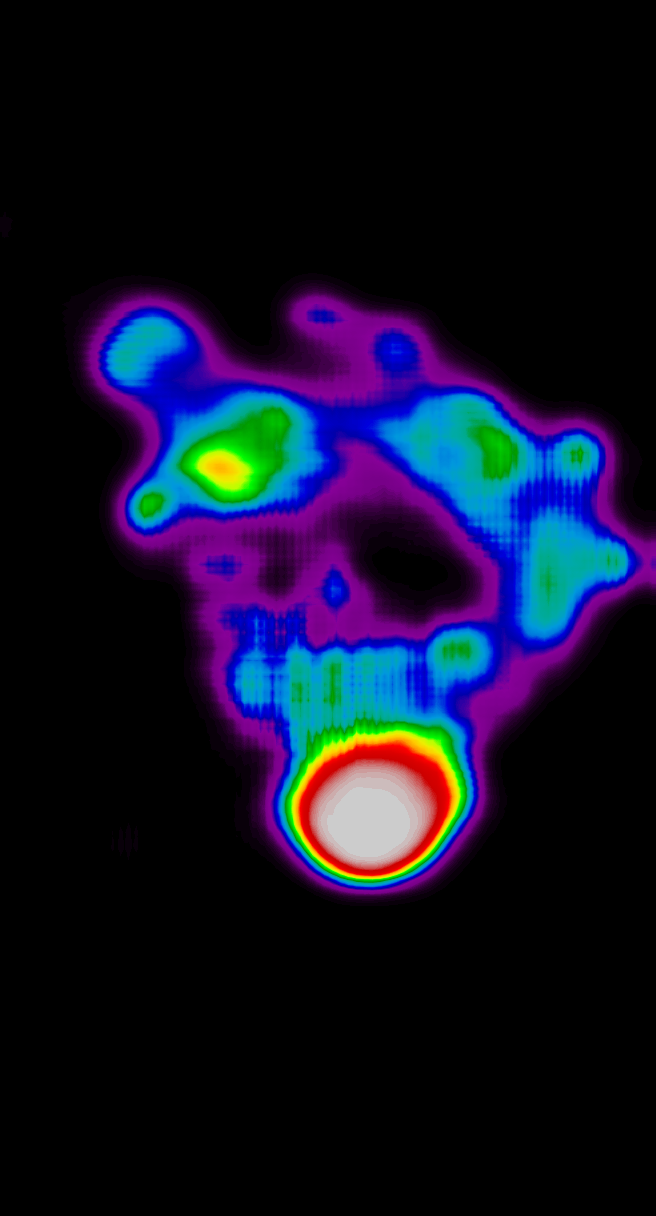
\includegraphics[width=\textwidth]{plots/examples/example5_probs_3.png}
		\caption{Experiment 3}
    \end{subfigure}
	\caption[Predictions for example 5]{Predicted probabilitites for example 5.}
\end{figure}
